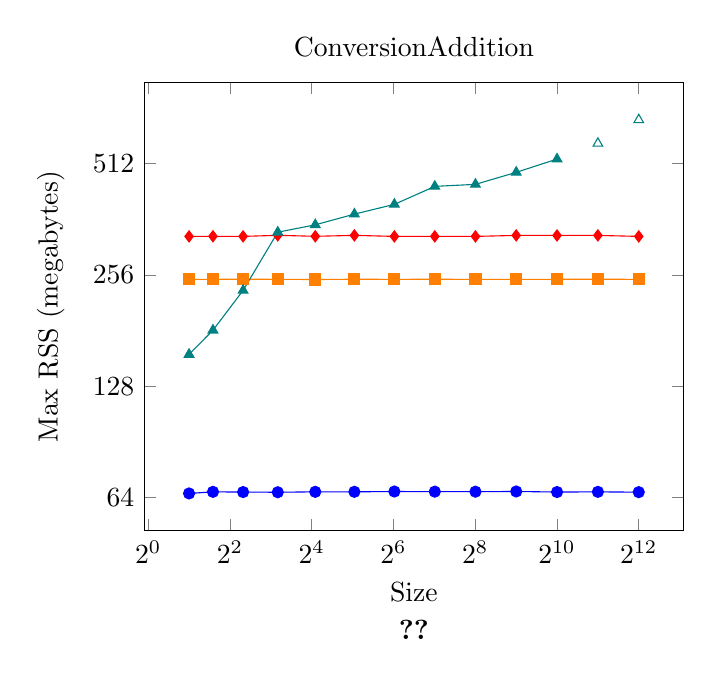
\begin{tikzpicture}
\begin{axis}
[title=ConversionAddition,
xlabel={Size},
ylabel={Max RSS (megabytes)},
legend to name=legend,
legend columns=2,
xmode=log,
log basis x={2},
ymode=log,
log basis y={2},
yticklabel={
  \pgfkeys{/pgf/fpu=true}
  \pgfmathparse{pow(2,\tick)}
  \pgfmathprintnumber[fixed relative,precision=3]{\pgfmathresult}
  \pgfkeys{/pgf/fpu=false}
}]
\addplot [
color=blue,
mark=o,
only marks,
forget plot
] coordinates {

};
\addplot [
color=orange,
mark=square,
only marks,
forget plot
] coordinates {

};
\addplot [
color=red,
mark=diamond,
only marks,
forget plot
] coordinates {

};
\addplot [
color=teal,
mark=triangle,
only marks,
forget plot
] coordinates {
(4097.0,670.814208) 
(2049.0,579.395584) 
};
\addplot [
color=blue,
mark=*
] coordinates {
(4097.0,66.215936) 
(2049.0,66.33472) 
(1025.0,66.265088) 
(513.0,66.494464) 
(257.0,66.408448) 
(129.0,66.428928) 
(65.0,66.47808) 
(33.0,66.3552) 
(17.0,66.347008) 
(9.0,66.179072) 
(5.0,66.2528) 
(3.0,66.338816) 
(2.0,65.691648) 
};
\addlegendentry{Agda}
\addplot [
color=orange,
mark=square*
] coordinates {
(4097.0,248.733696) 
(2049.0,248.950784) 
(1025.0,248.795136) 
(513.0,248.737792) 
(257.0,248.684544) 
(129.0,248.926208) 
(65.0,248.741888) 
(33.0,248.918016) 
(17.0,248.479744) 
(9.0,248.77056) 
(5.0,248.938496) 
(3.0,248.766464) 
(2.0,248.823808) 
};
\addlegendentry{Idris 2}
\addplot [
color=red,
mark=diamond*
] coordinates {
(4097.0,324.943872) 
(2049.0,326.897664) 
(1025.0,326.8608) 
(513.0,326.905856) 
(257.0,324.923392) 
(129.0,324.97664) 
(65.0,324.927488) 
(33.0,326.971392) 
(17.0,325.095424) 
(9.0,327.081984) 
(5.0,324.927488) 
(3.0,325.09952) 
(2.0,324.845568) 
};
\addlegendentry{Lean 4}
\addplot [
color=teal,
mark=triangle*
] coordinates {
(1025.0,525.53728) 
(513.0,483.926016) 
(257.0,449.097728) 
(129.0,443.465728) 
(65.0,396.525568) 
(33.0,373.219328) 
(17.0,349.188096) 
(9.0,333.508608) 
(5.0,232.206336) 
(3.0,181.313536) 
(2.0,155.938816) 
};
\addlegendentry{Rocq}
\end{axis}
\node[anchor=north] at (current axis.below south) {\ref{legend}};
\end{tikzpicture}
